%%%%%%%%%%%%%%%%%%%%%%%%%%%%%%%%%%%%%%%%%%%%%%%%%%%%%%%%%%%%%%%%%%%%%%%%%%%%%%%%%%
\begin{frame}[fragile]\frametitle{}
\begin{center}
{\Large Conclusions}
\end{center}
\end{frame}




%%%%%%%%%%%%%%%%%%%%%%%%%%%%%%%%%%%%%%%%%%%%%%%%%%%%%%%%%%%
\begin{frame}[fragile]\frametitle{Advantages}


\begin{itemize}
\item Conversational Abilities
\item Solving Complex Problems
\item Retaining Previous Information
\item Creative Assistant, random-mix-ideas
\item Will replace mundane language tasks, How to articles, homeworks, etc
\item Supports more complex instructions, ``reasoning'' tasks
\end{itemize}	 

\end{frame}

%%%%%%%%%%%%%%%%%%%%%%%%%%%%%%%%%%%%%%%%%%%%%%%%%%%%%%%%%%%
\begin{frame}[fragile]\frametitle{Dis-advantages}


\begin{itemize}
\item Sensitive to Input Phrasing
\item Incorrect Answers at Times
\item Cannot replace humans for innovation, for which data does not exist already
\item Keeps ``hallucinating''
\item Tends to write plausible but incorrect content with confidence
\item Cannot get language structure right all the time, e.g try getting ghazal written
\end{itemize}	 

\end{frame}



%%%%%%%%%%%%%%%%%%%%%%%%%%%%%%%%%%%%%%%%%%%%%%%%%%%%%%%%%%%
\begin{frame}[fragile]\frametitle{My Sketchnote}

\begin{center}
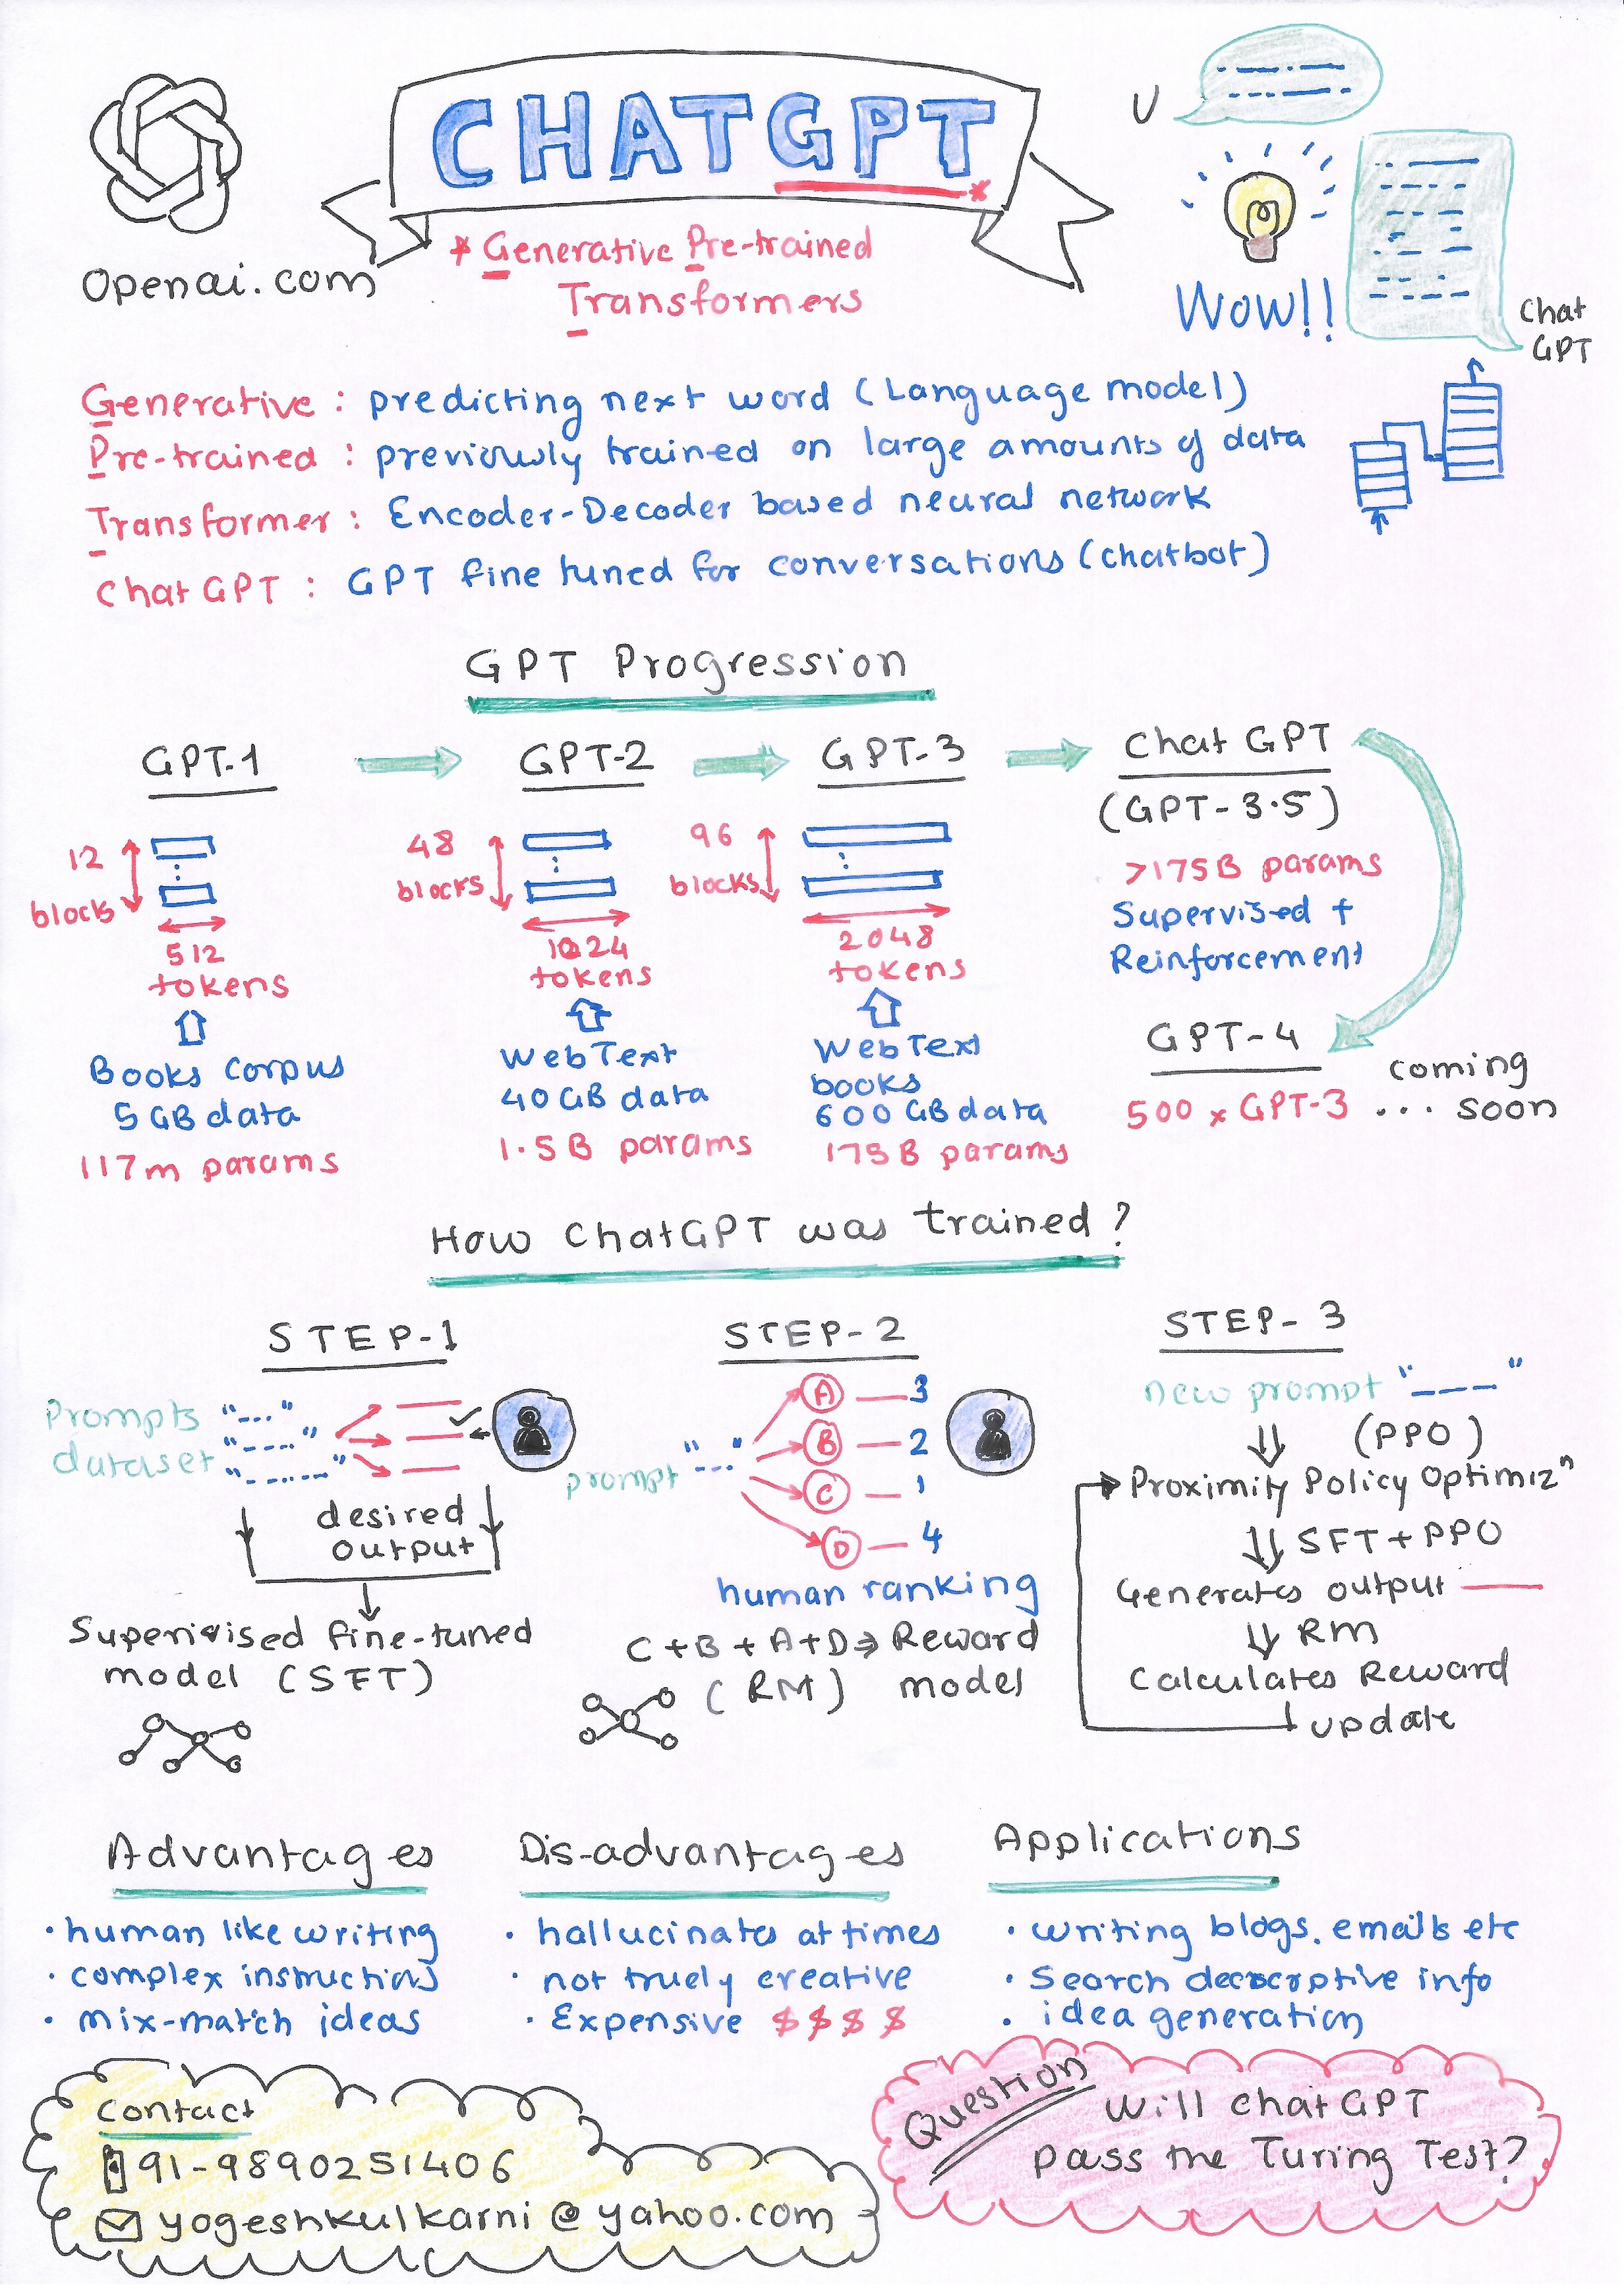
\includegraphics[width=0.45\linewidth,keepaspectratio]{ChatGPT_Sketchnote_Medium}
\end{center}		

{\tiny (Ref: https://medium.com/technology-hits/overview-of-chatgpt-95f4b43645c0)}
			

\end{frame}


%%%%%%%%%%%%%%%%%%%%%%%%%%%%%%%%%%%%%%%%%%%%%%%%%%%%%%%%%%%%%%%%%%%%%%%%%%%%%%%%%%
\begin{frame}[fragile]\frametitle{}
\begin{center}
{\Large The Effect}
\end{center}
\end{frame}



%%%%%%%%%%%%%%%%%%%%%%%%%%%%%%%%%%%%%%%%%%%%%%%%%%%%%%%%%%%
\begin{frame}[fragile]\frametitle{ChatGPT vs Google}


\begin{center}

\includegraphics[width=0.8\linewidth,keepaspectratio]{chatgpt28}
\end{center}		

Google: almost latest data, gives source, not trainable, looks more accurate
ChatGPT: a bit old data, no source, trainable, hallucinates

\tiny{(Ref:ChatGPT Explained: Complete A-Z Guide - Kripesh Adwani)}
\end{frame}


%%%%%%%%%%%%%%%%%%%%%%%%%%%%%%%%%%%%%%%%%%%%%%%%%%%%%%%%%%%
\begin{frame}[fragile]\frametitle{Will ChatGPT Kill Jobs?}


\begin{center}

\includegraphics[width=0.8\linewidth,keepaspectratio]{chatgpt29}
\end{center}		

Repetitive, boring and standard, language based jobs, for sure.
Need to be more creative, experiential to stand against ChatGPT.

\tiny{(Ref:ChatGPT Explained: Complete A-Z Guide - Kripesh Adwani)}
\end{frame}


%%%%%%%%%%%%%%%%%%%%%%%%%%%%%%%%%%%%%%%%%%%%%%%%%%%%%%%%%%%%%%%%%%%%%%%%%%%%%%%%%%
\begin{frame}[fragile]\frametitle{New Job Roles?}
Prompt Engineer: Preparing input to AI effectively to get the desired answer. Will need to AI works in the background plus domain knowledge. Give context, examples etc to prime the model to give short specific answers than the usual page-long ones (davinci GPT3 in this case)

			\begin{center}
			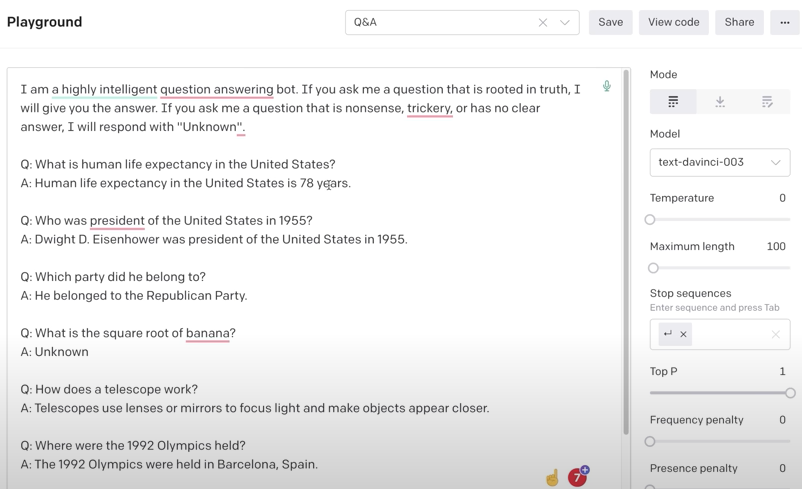
\includegraphics[width=0.8\linewidth,keepaspectratio]{chatgpt11}
			
			\end{center}		
			
			{\tiny (Ref: Advanced ChatGPT Guide - How to build your own Chat GPT Site - Drian Twarog)}
			

\end{frame}

% %%%%%%%%%%%%%%%%%%%%%%%%%%%%%%%%%%%%%%%%%%%%%%%%%%%%%%%%%%%
% \begin{frame}[fragile]\frametitle{Whats happening around, now?}


% \begin{itemize}
% \item ``Science journals ban listing of ChatGPT as co-author on papers'' - The Guardian
% \item OpenAI’s ChatGPT Took An IQ Test! - Two Minutes Papers
% \item Discussing internally as one of the Editors on a Medium Publication, that Do we allow AI generated articles? and if yes, how?
% \item Google’s DeepMind might release ChatGPT competitor Sparrow this year
% \end{itemize}	 

% \end{frame}

%%%%%%%%%%%%%%%%%%%%%%%%%%%%%%%%%%%%%%%%%%%%%%%%%%%%%%%%%%%
\begin{frame}[fragile]\frametitle{The Hype}


\begin{center}
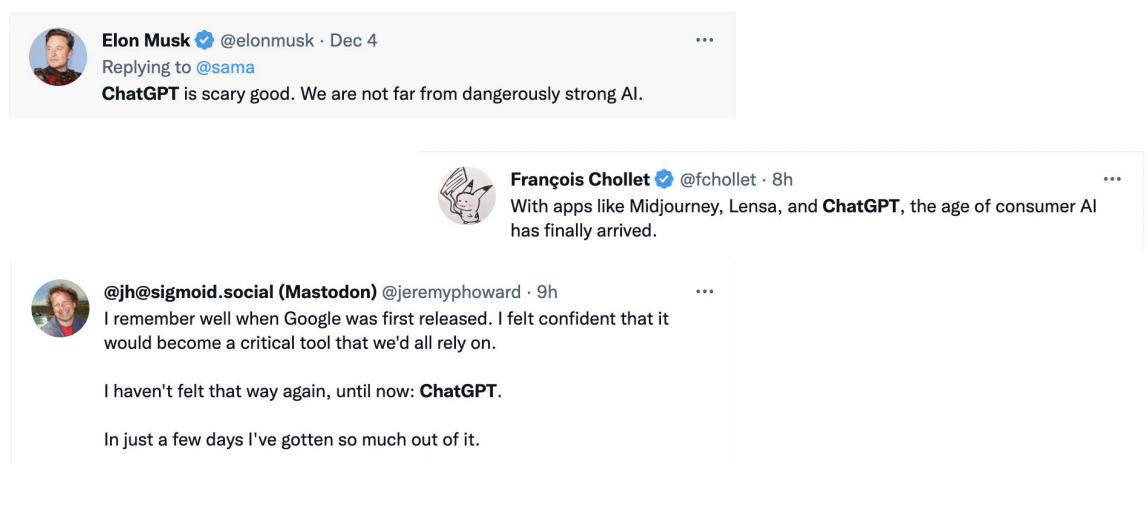
\includegraphics[width=\linewidth,keepaspectratio]{chatgpt32}
\end{center}		

{\tiny (Ref: ChatGPT - Intro \& Potential Impact Sudalai Rajkumar, SRK)}
			

\end{frame}



%%%%%%%%%%%%%%%%%%%%%%%%%%%%%%%%%%%%%%%%%%%%%%%%%%%%%%%%%%%
\begin{frame}[fragile]\frametitle{Finally, from horses mouth!!}


\begin{center}
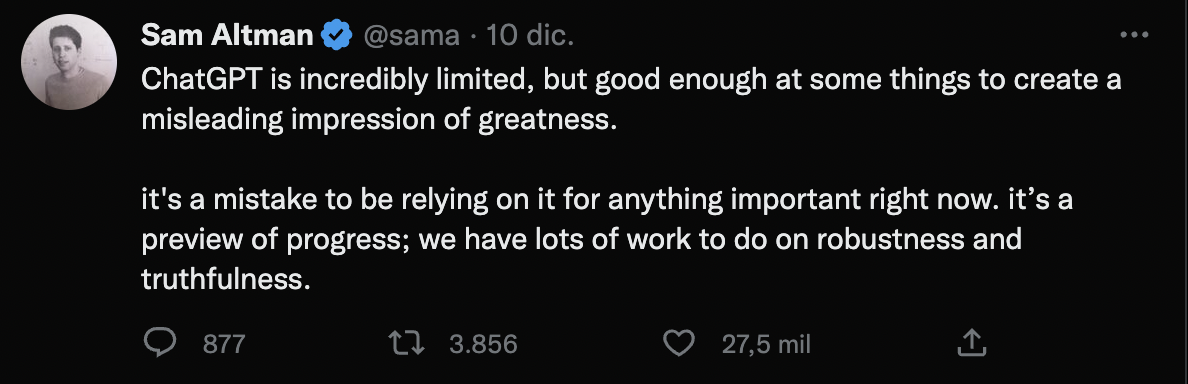
\includegraphics[width=\linewidth,keepaspectratio]{chatgpt7}
\end{center}		

{\tiny (Ref: ChatGPT: training process, advantages, and limitations - By Sergio Soage, Machine Learning Engineer at Aivo)}
			

\end{frame}

% %%%%%%%%%%%%%%%%%%%%%%%%%%%%%%%%%%%%%%%%%%%%%%%%%%%%%%%%%%%
% \begin{frame}[fragile]\frametitle{Whats next? - GPT4 }


% \begin{center}
% 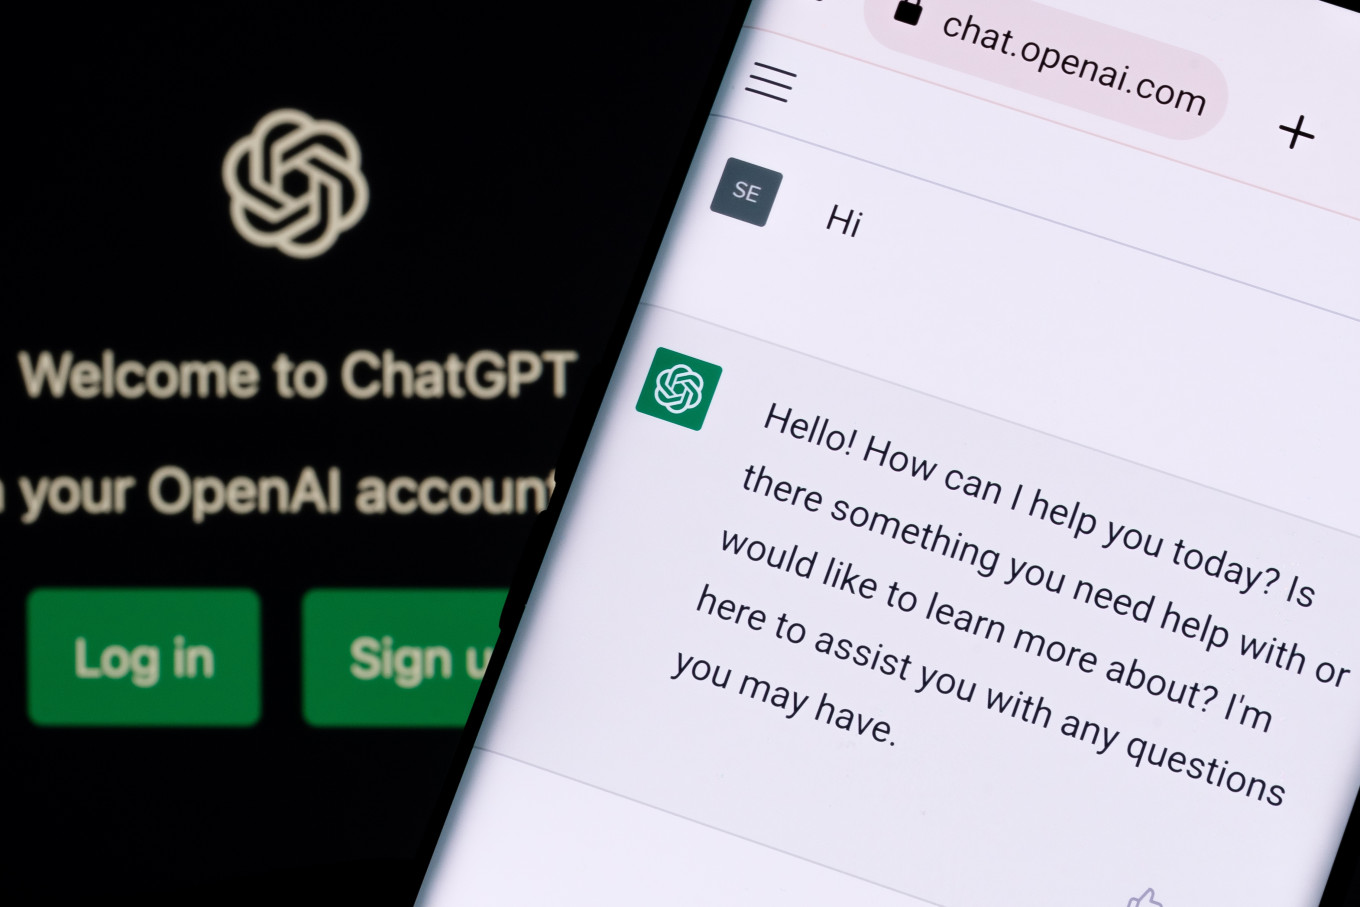
\includegraphics[width=\linewidth,keepaspectratio]{chatgpt33}
% \end{center}		

% *not confirmed yet

% {\tiny (Ref: https://twitter.com/WolfofBaldSt/status/1596768686051921923)}
			

% \end{frame}


%%%%%%%%%%%%%%%%%%%%%%%%%%%%%%%%%%%%%%%%%%%%%%%%%%%%%%%%%%%
\begin{frame}[fragile]\frametitle{References}
		\begin{itemize}
		\item Let's build GPT: from scratch, in code, spelled out: Andrej Karpathy
		\item ChatGPT and Reinforcement Learning - CodeEmporium
		\end{itemize}
\end{frame}
